\chapter{Regularization}

\section{The Problem of Overfitting}

Consider the problem of predicting y from x $\in$ $ \mathbb{R} $. The leftmost figure below shows the result of fitting a $ y = \theta_0+\theta_1x $ to a dataset. We see that the data doesn’t really lie on straight line, and so the fit is not very good.\\

Instead, if we had added an extra feature $ x^2 $, and fit $ y = \theta_0 + \theta_1x + \theta_2x^2 $, then we obtain a slightly better fit to the data (See middle figure). Naively, it might seem that the more features we add, the better. However, there is also a danger in adding too many features: The rightmost figure is the result of fitting a $ 5^{th} $order polynomial $$ y = \sum_{j=0} ^5 \theta_j x^j .$$ We see that even though the fitted curve passes through the data perfectly, we would not expect this to be a very good predictor of, say, housing prices (y) for different living areas (x). Without formally defining what these terms mean, we’ll say the \textit{figure on the left} shows an instance of \textbf{underfitting}—in which the data clearly shows structure not captured by the model—and the \textit{figure on the right} is an example of \textbf{overfitting}.

\begin{figure}[h!]
	\centering
	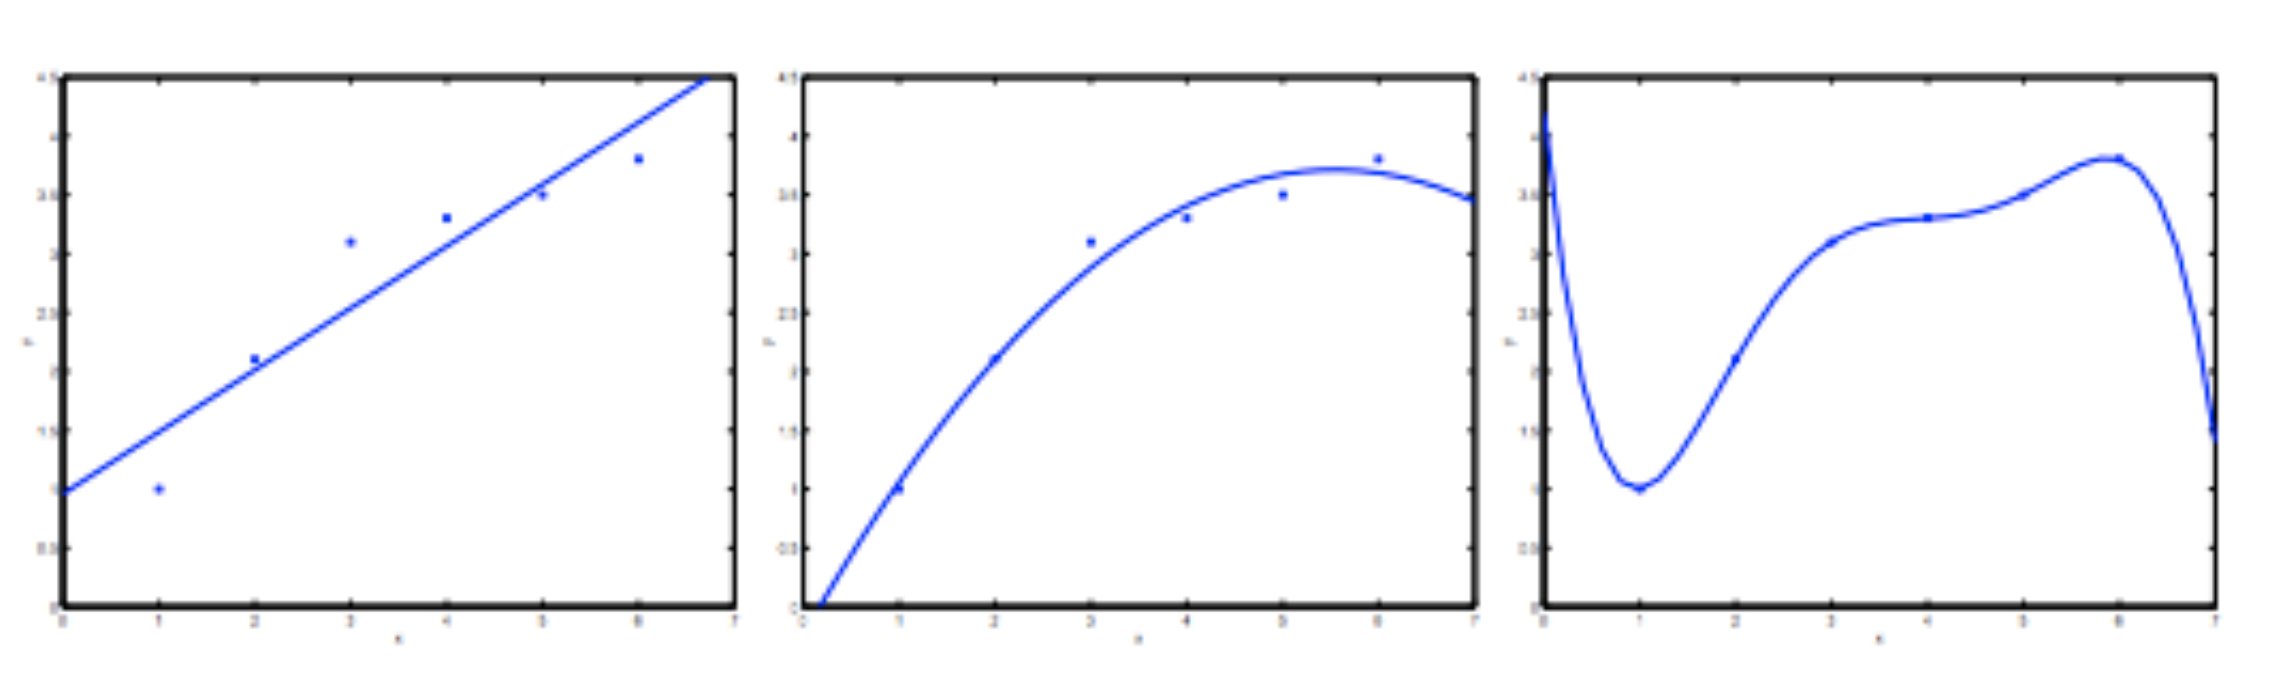
\includegraphics[width=1\textwidth]{fig/regula}
	\caption{One-vs-all or One-vs-Rest}
\end{figure}

\textbf{Underfitting, or high bias}, is when the form of our hypothesis function h maps poorly to the trend of the data.\\

\textbf{Overfitting, or high variance}, is caused by a hypothesis function that fits the available data but does not generalize well to predict new data.\\

This terminology is applied to both linear and logistic regression. There are two main options to address the issue of overfitting:\\

\begin{enumerate}
\item Reduce the number of features: Manually select which features to keep; Use a model selection algorithm.
\item Regularization: Keep all the features, but reduce the magnitude of parameters $ \theta_j $. Regularization works well when we have a lot of slightly useful features.
\end{enumerate}

\section{Cost Function}

Say we wanted to make the following function more quadratic:

\begin{center}
$ y = \theta_0 + \theta_1x + \theta_2x^2 + \theta_3x^3 + \theta_4x^4$
\end{center}

We'll want to eliminate the influence of $ \theta_3x^3 $and $ \theta_4x^4 $ without actually getting rid of these features or changing the form of our hypothesis, we can instead modify our cost function:\\

\begin{center}
$$min_\theta   \frac{1}{2m}\sum_{i=1}^{m}\left(h_\theta(x^{(i)}) - y^{(i)}\right)^2 + 1000\cdot \theta_3x^3 + 1000\cdot \theta_4x^4 $$
\end{center}

We've added two extra terms at the end to inflate the cost of $ \theta_3 $and $ \theta_4 $. Now, in order for the cost function to get close to zero, we will have to reduce the values of $ \theta_3 $and $ \theta_4 $ to near zero. This will in turn greatly reduce the values of $ \theta_3 x^3 $and $ \theta_4x^4 $ in our hypothesis function.\\

\subsection{Linear Regression}

We could also regularize all of our theta parameters in a single summation as:\\

\begin{center}
	$$min_\theta   \frac{1}{2m}\sum_{i=1}^{m}\left(h_\theta(x^{(i)}) - y^{(i)}\right)^2 + \lambda  \sum_{i=1}^{n} \theta_j^2$$
\end{center}

The lambda is the regularization parameter. It determines how much the costs of our theta parameters are inflated.

\subsection{Logistic Regression}

\begin{center}
	$$J(\theta) = -\frac{1}{m}\sum_{i=1}^{m}\left[y^{(i)}\cdot log(h_\theta(x^{(i)})) +(1-y^{(i)})\cdot log(1-h_\theta(x^{(i)}))\right] + \frac{\lambda}{2m}  \sum_{i=1}^{n} \theta_j^2$$
\end{center}

The second sum, $$\sum_{i=1}^{n} \theta_j^2$$ means to explicitly exclude the bias term, $ \theta_0 $. I.e. the $ \theta $ vector is indexed from 0 to n (holding n+1 values, $ \theta_0 $ through $ \theta_n $), and this sum explicitly skips $ \theta_0 $, by running from 1 to n, skipping 0. (\textbf{Identically for linear regression}).

\section{Gradient Descent}

We will modify our gradient descent function to separate out $ \theta_0 $ from the rest of the parameters because we do not want to penalize $ \theta_0 $.

\begin{align*}
Repeat &: \{\\
\theta_0 &:= \theta_0-\alpha \frac{1}{m} \sum_{i=1}^{m}\left(h_\theta(x^{(i)})-y^{(i)}\right)\cdot x^{(i)}_0\\
\theta_j &:= \theta_j-\alpha \left[ \left(\frac{1}{m} \sum_{i=1}^{m}\left(h_\theta(x^{(i)})-y^{(i)}\right)\cdot x^{(i)}_j  \right) +\frac{\lambda}{m}\theta_j\right] \hspace{1cm} j \in \{1,2, \dots, n\}\\
&   \}
\end{align*}

\section{Normal Equation}

Now let's approach regularization using the alternate method of the non-iterative normal equation.\\

To add in regularization, the equation is the same as our original, except that we add another term inside the parentheses:\\

\begin{center}
$\theta = (X^TX+\lambda\cdot L)^{-1} X^Ty$
\end{center}

Where:

\[
L =
\begin{bmatrix}
0 & && &\\
& 1& & &\\
& & 1&&\\
&&&\ddots&\\
&&&&1
\end{bmatrix}
\]

L is a matrix with 0 at the top left and 1's down the diagonal, with 0's everywhere else. It should have dimension (n+1)x(n+1).